\section{Supported Changes}
\label{sec:supported-changes}

We have designed a simple, yet flexible update model that supports updates
that we have seen to be common in practice.

\paragraph{Method body changes}
Programmers may change method bodies. Method body updates are the simplest
and most commonly supported change~\cite{JVMhotswap, VSEnC, eaddy05enc,
GilmoreKW97, orso:java, K42reconfig, HjalmtyssonG98}. DSU systems
can preserve type safety by simply invoking the new method the next time
the program executes the method. However, restricting updates to only method
bodies prevents many common changes~\cite{neamtiu05evolution}.
Chapter~\ref{chap:experience} shows that over half the releases of Jetty,
JavaEmailServer, and CrossFTP, the programs we studied, change more than method bodies.

\paragraph{Class signature changes}
Programmers may also change class signatures in various ways.
% By class signature, we mean the interface a class exposes to other classes and
% methods.
The class signature includes all fields and methods defined by the class
and those inherited from super classes. A programmer may change method
signatures by changing the type or number of method arguments. They
may add or delete virtual and static field members, and change the types or
access modifiers of existing members.  These changes may occur at any level
of the class hierarchy.  For example, programmers may delete a field from a
parent class and this change will propagate correctly to the class's
descendants.
% We rely on the bytecode compiler to ensure that the resulting
% program is type-safe, and thus there are no more accesses to the deleted field
% in the program.  

\begin{figure}[t]
\begin{tabular}{@{}m{0.5\textwidth}@{}m{0.5\textwidth}@{}}
\BC \begin{minipage}{0.4\textwidth}
\begin{lstlisting}
private int x;
private static int y;
public int getX();
public static int getY();
\end{lstlisting}
\end{minipage} \EC &
\BC \begin{minipage}{0.45\textwidth}
\begin{lstlisting}
private double x;
private static double y;
public double getX();
public static double getY();
\end{lstlisting}
\end{minipage} \EC \\[-2ex]
\BC (a) Old version \EC &
\BC (b) New version \EC \\[-2ex]
\end{tabular}
\caption{Examples of an update that changes class signature}
\label{fig:class-sig-change-example}
\end{figure}


\begin{figure}[p]
\BC \begin{minipage}{0.92\textwidth}
\begin{lstlisting}[frame=single]
public class User {
  private final String username, domain, password;
  private String[] forwardAddresses;
  public User(...) {...}
  public String[] getForwardedAddresses() {...}
  public void setForwardedAddresses(String[] f) {...}
}
public class ConfigurationManager {
  private User loadUser(...) {
     ...
     User user = new User(...);
     String[] f = ...;
     user.setForwardedAddresses(f);
     return user;
  }
}
\end{lstlisting}
\end{minipage} \\
(a) Version 1.3.1 \EC

\BC \begin{minipage}{0.92\textwidth}
\begin{lstlisting}[frame=single]
public class User {
  private final String username, domain, password;
  private EmailAddress[] forwardAddresses;
  public User(...) {...}
  public EmailAddress[] getForwardedAddresses() {...}
  public void setForwardedAddresses(EmailAddress[] f) {...}
}
public class ConfigurationManager {
  private User loadUser(...) {
     ...
     User user = new User(...);
     EmailAddress[] f = ...;
     user.setForwardedAddresses(f);
     return user;
  }
}
\end{lstlisting}
\end{minipage} \\
(b) Version 1.3.2 \EC
\hangcaption{Changes to JavaEmailServer \User and {\tt
ConfigurationManager} classes from version 1.3.1 to version 1.3.2}
\label{fig:jes-string-emailaddress-example}
\end{figure}


Figure~\ref{fig:class-sig-change-example} provides examples of class
signature changes. Each line in the figure defines either a field or a
method and represents a class signature change in the new version.
Internally, \UPT does not view this update as changing the signature of
individual fields and methods. Instead, it views the update as removing the
field {\tt int x} and adding a new field {\tt double x}, and similarly for
the methods. Irrespective of how \UPT views this change, it is pertinent to
note that any reference to these fields and methods in the new version must
conform to the new type signature. The Java to bytecode compiler
will ensure that the standalone new version of the program is well-formed.

\JV does not support permutations of the class hierarchy, e.g., reversing
a super-class relationship.  While this change may be desirable in
principle, in practice, it requires sophisticated transformers that enforce
update ordering constraints. None of the program versions we examined make
this type of change. \JV also does not support renaming a class, though
this functionality should be easy to add.
% While it
% is not hard to implement this support, we did not 

% In summary, \UPT recognizes changes with method bodies and changes that add
% or remove fields or methods.

\paragraph{Example.} Consider the following update from JavaEmailServer, a
simple SMTP and POP e-mail server.
Figure~\ref{fig:jes-string-emailaddress-example} illustrates a pair of
classes that change between versions 1.3.1 and 1.3.2.  \JV fully supports
these changes. JavaEmailServer uses the class \User to maintain information
about e-mail user accounts in the server.  Moving from version 1.3.1 to
1.3.2, there are three differences. First, the method {\tt loadUser} fixes
some problems with the loading of forwarded addresses from a configuration
file (details not shown). This change is a simple method update.  Second,
the array of forwarded addresses in the new version contains instances of a
new class, {\tt EmailAddress}, rather than {\tt String}.  This change
modifies the class signature of \User since it modifies the type of {\tt
forwardedAddresses}. Finally, the class's {\tt setForwardedAddresses}
method is also altered to take an array of {\tt EmailAddress}es instead of
an array of {\tt String}s, and code from {\tt loadUser} accommodates this
change as well.

\section{VM object model and method dispatch}
\label{sec:dsu-view-of-changes}
\JV's dynamic application of an update closely follows \UPT's static specification, and
is related to how a
\JVM would support field accesses and method calls. In
languages such as C and Java accessing a field involves reading to or
writing from an offset from a structure or object's address. This offset is
determined at compile-time. In a language like Java, by compile-time we
mean the time when bytecode is translated to machine code. Method calls in
C, involve jumping to a memory location that contains the machine code for
the called method. Method calls in Java are similar, except that a \JVM
needs to support \emph{virtual method dispatch}. There can be different
definitions of the same method and which one is invoked depends on the
object in hand. \JVM{}s use \aclp{VMT} which contain pointers to compiled
machine codes of methods. A method call looks up the contents of a particular
slot in the \VMT and jumps to that address.

\begin{figure}[p]
\lstset{frame=single}
\begin{tabular}[t]{@{}c@{ }c@{}}
\begin{minipage}{0.35\textwidth}
\begin{lstlisting}
public class A {
  private int x, y;
  public void f() {
    g();
  };
  public void g() {
    this.y = 0;
  }
}

public class B
          extends A {
  private int z;
  public void g() {
    this.z = 0;
  }
  public void h() {}
}
\end{lstlisting}
\end{minipage}
&
\begin{minipage}{0.64\textwidth}
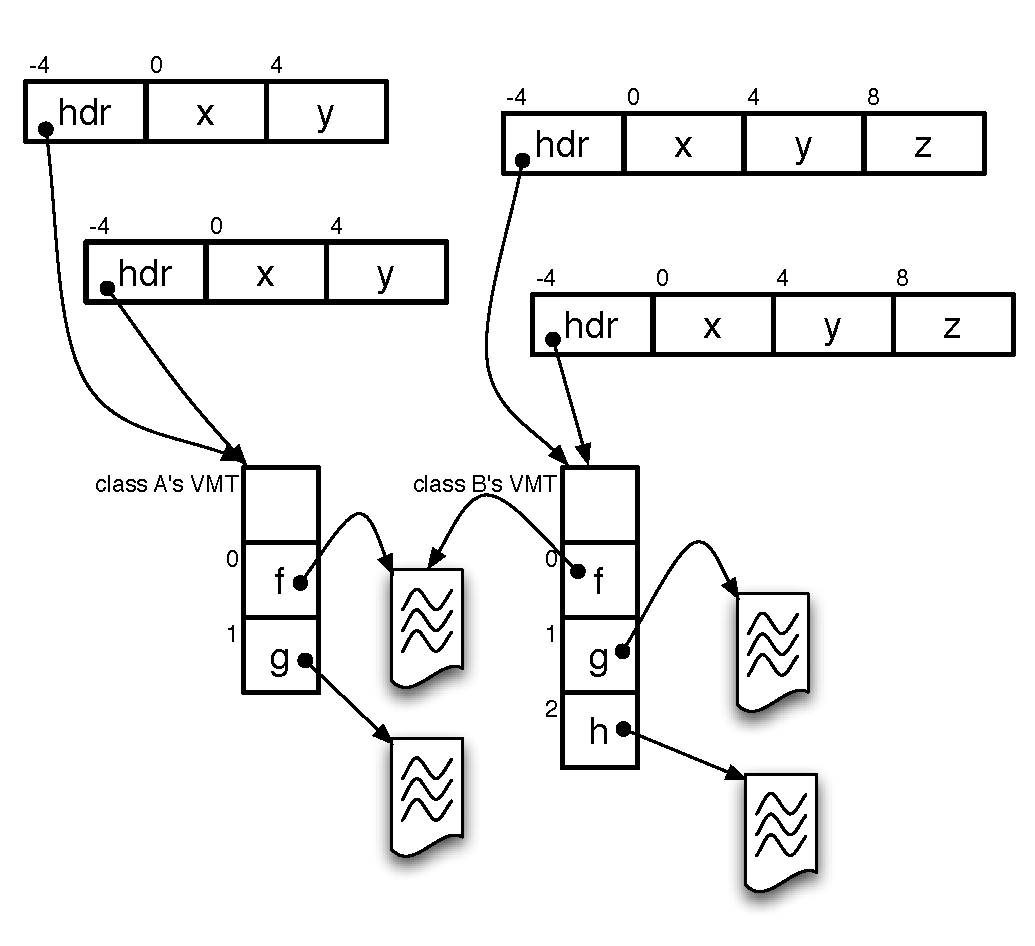
\includegraphics[draft=false,scale=0.5]{100-images/field-method-access-explanation}
\end{minipage} \\
\begin{minipage}{0.28\textwidth}
(a) Java source code
\end{minipage} &
\begin{minipage}{0.44\textwidth}
(b) Objects and VMTs in the heap
\end{minipage} \\[2ex]
\begin{minipage}{0.35\textwidth}
\begin{lstlisting}
aload_0
invokevirtual <A.g>
return
\end{lstlisting}
\vspace{-2ex}
\BC (a) Bytecode for A.f() \EC
\end{minipage} &
\begin{minipage}{0.55\textwidth}
\lstset{moredelim=[il][commentstyle]{>}}
\begin{lstlisting}
>The stack pointer points to "this"
>EDX := this
        MOV     EDX      [ESP]
>The VMT is at offset -4
>ECS := VMT
        MOV     ECX   -4[EDX]
>Send this parameter in EAX
>EAX := this
        MOV     EAX      [ESP]
>Call function g()
>g() is at offset 8 within VMT
        CALL 8[ECX]
\end{lstlisting}
\end{minipage} \\
% \begin{minipage}{0.28\textwidth}
% (c) Bytecode for A.f()
% \end{minipage} &
&
\begin{minipage}{0.38\textwidth}
(d) Machine code for the {\tt invokevirtual} instruction
\end{minipage} \\
\end{tabular}
\hangcaption{Simple example of method and field accesses to illustrate how
inheritance is implemented in Java}
\label{fig:field-method-access-explanation}
\lstset{frame=none}
\end{figure}


We illustrate how a typical VM supports field accesses and method calls
with a simple example shown in
Figure~\ref{fig:field-method-access-explanation}. The class {\tt A} defines two
integer fields {\tt x} and {\tt y}. Objects of type {\tt A} have these
fields laid out contiguously. Objects of {\tt class B} have an additional
integer field {\tt z}. In managed languages, the runtime system maintains a header
field for all objects, which it uses to look up at runtime the type of a particular
object instance. The runtime also uses the object header to look up the
type's \VMT to invoke methods.
{\tt class A}'s
\VMT has method {\tt f()} at slot 0 and method {\tt g()} at slot 1. The
class
{\tt B} overrides method {\tt g()}. In addition, {\tt class B} defines a
new method {\tt h()} that takes slot 2.
Figure~\ref{fig:field-method-access-explanation}~(b) shows
\VMT{}s of {\tt A} and {\tt B}. \VMT slots point to compiled machine code
of respective methods. {\tt A.f()} and {\tt B.f()} both point to the same
code, while {\tt A.g()} and {\tt B.g()} point to different methods since
{\tt B} overrides {\tt g()}. The figure also shows objects of type {\tt A} and
{\tt B}.  The header field of these objects (chosen arbitrarily to be
at offset -4) allow access to their respective \VMT{}s.

Figure~\ref{fig:field-method-access-explanation}~(d) shows function {\tt
f()}'s generated machine code. The call to {\tt g()} refers to \VMT slot 1
(at offset 8). This call invokes either {\tt A.g()} or {\tt B.g()} based on
the type of the object making the call.  Whenever the \VMT slot of a method
is known at compile time, callers of that method use the offset in their
machine code. Similarly, the machine code usually contains offsets of
fields as well --- for instance, functions {\tt A.g()} and {\tt B.g()}
referring to offsets for {\tt y} and {\tt z} respectively. The interface a \VM
presents to the compiler consists of the following --- \acl{VMT} with methods
at various slots, and objects with fields laid out at various offsets.

\section{\JV's view of updates}

\JV groups updates presented by the \UPT into two categories --- those that
change the exposed representation of a class, and those that don't. \JV
handles updates as follows.
\begin{itemize}
\item Method body changes: \JV invalidates any old machine code, loads the
new bytecode of the method, and lazily generates new machine code.
\item Class signature changes:
  \begin{enumerate}
  \item The update changes the number and offsets of fields within an object. \JV creates
        new object instances that conform to the layout of the new version
        and copies fields appropriately. \JV also needs to initialize
        fields that do not exist in the old version.
        Section~\ref{subsec:transformers}
        talks about such changes and how \JV transforms objects to conform
        to the semantics of the application.
  \item The update changes the number and offsets of method slots in a class' \acl{VMT}. \JV
        creates new \VMT{}s and points all object instances to this new \VMT.
  \end{enumerate}
\item Methods that are not changed by the update but that refer to classes
with signature changes. The machine code of such methods will have field
and method offsets that are invalid in the new version. \JV invalidates old
codes, and lazily recompiles
such methods to generate machine code afresh. We refer to such methods as
\emph{indirect updates}.
\end{itemize}

\JV, with respect to the implementation of dynamic updating, does not view
classes as monolithic collections of fields and methods. Instead it views
them as method bodies that need to be updated, and structure instances
whose fields need to be aligned and have proper values to conform to the
semantics of the new version.
